\documentclass{ximera}

%\usepackage{todonotes}

\newcommand{\todo}{}

\usepackage{esint} % for \oiint
\ifxake%%https://math.meta.stackexchange.com/questions/9973/how-do-you-render-a-closed-surface-double-integral
\renewcommand{\oiint}{{\large\bigcirc}\kern-1.56em\iint}
\fi


\graphicspath{
  {./}
  {ximeraTutorial/}
  {basicPhilosophy/}
  {functionsOfSeveralVariables/}
  {normalVectors/}
  {lagrangeMultipliers/}
  {vectorFields/}
  {greensTheorem/}
  {shapeOfThingsToCome/}
  {dotProducts/}
  {partialDerivativesAndTheGradientVector/}
  {../productAndQuotientRules/exercises/}
  {../normalVectors/exercisesParametricPlots/}
  {../continuityOfFunctionsOfSeveralVariables/exercises/}
  {../partialDerivativesAndTheGradientVector/exercises/}
  {../directionalDerivativeAndChainRule/exercises/}
  {../commonCoordinates/exercisesCylindricalCoordinates/}
  {../commonCoordinates/exercisesSphericalCoordinates/}
  {../greensTheorem/exercisesCurlAndLineIntegrals/}
  {../greensTheorem/exercisesDivergenceAndLineIntegrals/}
  {../shapeOfThingsToCome/exercisesDivergenceTheorem/}
  {../greensTheorem/}
  {../shapeOfThingsToCome/}
  {../separableDifferentialEquations/exercises/}
}

\newcommand{\mooculus}{\textsf{\textbf{MOOC}\textnormal{\textsf{ULUS}}}}

\usepackage{tkz-euclide}\usepackage{tikz}
\usepackage{tikz-cd}
\usetikzlibrary{arrows}
\tikzset{>=stealth,commutative diagrams/.cd,
  arrow style=tikz,diagrams={>=stealth}} %% cool arrow head
\tikzset{shorten <>/.style={ shorten >=#1, shorten <=#1 } } %% allows shorter vectors

\usetikzlibrary{backgrounds} %% for boxes around graphs
\usetikzlibrary{shapes,positioning}  %% Clouds and stars
\usetikzlibrary{matrix} %% for matrix
\usepackage{pgfplots}
\usepgfplotslibrary{polar} %% for polar plots
\usepgfplotslibrary{fillbetween} %% to shade area between curves in TikZ
\usetkzobj{all}
\usepackage[makeroom]{cancel} %% for strike outs
%\usepackage{mathtools} %% for pretty underbrace % Breaks Ximera
%\usepackage{multicol}
\usepackage{pgffor} %% required for integral for loops



%% http://tex.stackexchange.com/questions/66490/drawing-a-tikz-arc-specifying-the-center
%% Draws beach ball
\tikzset{pics/carc/.style args={#1:#2:#3}{code={\draw[pic actions] (#1:#3) arc(#1:#2:#3);}}}



\usepackage{array}
\setlength{\extrarowheight}{+.1cm}
\newdimen\digitwidth
\settowidth\digitwidth{9}
\def\divrule#1#2{
\noalign{\moveright#1\digitwidth
\vbox{\hrule width#2\digitwidth}}}





\newcommand{\RR}{\mathbb R}
\newcommand{\R}{\mathbb R}
\newcommand{\N}{\mathbb N}
\newcommand{\Z}{\mathbb Z}

\newcommand{\sagemath}{\textsf{SageMath}}


%\renewcommand{\d}{\,d\!}
\renewcommand{\d}{\mathop{}\!d}
\newcommand{\dd}[2][]{\frac{\d #1}{\d #2}}
\newcommand{\pp}[2][]{\frac{\partial #1}{\partial #2}}
\renewcommand{\l}{\ell}
\newcommand{\ddx}{\frac{d}{\d x}}

\newcommand{\zeroOverZero}{\ensuremath{\boldsymbol{\tfrac{0}{0}}}}
\newcommand{\inftyOverInfty}{\ensuremath{\boldsymbol{\tfrac{\infty}{\infty}}}}
\newcommand{\zeroOverInfty}{\ensuremath{\boldsymbol{\tfrac{0}{\infty}}}}
\newcommand{\zeroTimesInfty}{\ensuremath{\small\boldsymbol{0\cdot \infty}}}
\newcommand{\inftyMinusInfty}{\ensuremath{\small\boldsymbol{\infty - \infty}}}
\newcommand{\oneToInfty}{\ensuremath{\boldsymbol{1^\infty}}}
\newcommand{\zeroToZero}{\ensuremath{\boldsymbol{0^0}}}
\newcommand{\inftyToZero}{\ensuremath{\boldsymbol{\infty^0}}}



\newcommand{\numOverZero}{\ensuremath{\boldsymbol{\tfrac{\#}{0}}}}
\newcommand{\dfn}{\textbf}
%\newcommand{\unit}{\,\mathrm}
\newcommand{\unit}{\mathop{}\!\mathrm}
\newcommand{\eval}[1]{\bigg[ #1 \bigg]}
\newcommand{\seq}[1]{\left( #1 \right)}
\renewcommand{\epsilon}{\varepsilon}
\renewcommand{\phi}{\varphi}


\renewcommand{\iff}{\Leftrightarrow}

\DeclareMathOperator{\arccot}{arccot}
\DeclareMathOperator{\arcsec}{arcsec}
\DeclareMathOperator{\arccsc}{arccsc}
\DeclareMathOperator{\si}{Si}
\DeclareMathOperator{\scal}{scal}
\DeclareMathOperator{\sign}{sign}


%% \newcommand{\tightoverset}[2]{% for arrow vec
%%   \mathop{#2}\limits^{\vbox to -.5ex{\kern-0.75ex\hbox{$#1$}\vss}}}
\newcommand{\arrowvec}[1]{{\overset{\rightharpoonup}{#1}}}
%\renewcommand{\vec}[1]{\arrowvec{\mathbf{#1}}}
\renewcommand{\vec}[1]{{\overset{\boldsymbol{\rightharpoonup}}{\mathbf{#1}}}}
\DeclareMathOperator{\proj}{\mathbf{proj}}
\newcommand{\veci}{{\boldsymbol{\hat{\imath}}}}
\newcommand{\vecj}{{\boldsymbol{\hat{\jmath}}}}
\newcommand{\veck}{{\boldsymbol{\hat{k}}}}
\newcommand{\vecl}{\vec{\boldsymbol{\l}}}
\newcommand{\uvec}[1]{\mathbf{\hat{#1}}}
\newcommand{\utan}{\mathbf{\hat{t}}}
\newcommand{\unormal}{\mathbf{\hat{n}}}
\newcommand{\ubinormal}{\mathbf{\hat{b}}}

\newcommand{\dotp}{\bullet}
\newcommand{\cross}{\boldsymbol\times}
\newcommand{\grad}{\boldsymbol\nabla}
\newcommand{\divergence}{\grad\dotp}
\newcommand{\curl}{\grad\cross}
%\DeclareMathOperator{\divergence}{divergence}
%\DeclareMathOperator{\curl}[1]{\grad\cross #1}
\newcommand{\lto}{\mathop{\longrightarrow\,}\limits}

\renewcommand{\bar}{\overline}

\colorlet{textColor}{black}
\colorlet{background}{white}
\colorlet{penColor}{blue!50!black} % Color of a curve in a plot
\colorlet{penColor2}{red!50!black}% Color of a curve in a plot
\colorlet{penColor3}{red!50!blue} % Color of a curve in a plot
\colorlet{penColor4}{green!50!black} % Color of a curve in a plot
\colorlet{penColor5}{orange!80!black} % Color of a curve in a plot
\colorlet{penColor6}{yellow!70!black} % Color of a curve in a plot
\colorlet{fill1}{penColor!20} % Color of fill in a plot
\colorlet{fill2}{penColor2!20} % Color of fill in a plot
\colorlet{fillp}{fill1} % Color of positive area
\colorlet{filln}{penColor2!20} % Color of negative area
\colorlet{fill3}{penColor3!20} % Fill
\colorlet{fill4}{penColor4!20} % Fill
\colorlet{fill5}{penColor5!20} % Fill
\colorlet{gridColor}{gray!50} % Color of grid in a plot

\newcommand{\surfaceColor}{violet}
\newcommand{\surfaceColorTwo}{redyellow}
\newcommand{\sliceColor}{greenyellow}




\pgfmathdeclarefunction{gauss}{2}{% gives gaussian
  \pgfmathparse{1/(#2*sqrt(2*pi))*exp(-((x-#1)^2)/(2*#2^2))}%
}


%%%%%%%%%%%%%
%% Vectors
%%%%%%%%%%%%%

%% Simple horiz vectors
\renewcommand{\vector}[1]{\left\langle #1\right\rangle}


%% %% Complex Horiz Vectors with angle brackets
%% \makeatletter
%% \renewcommand{\vector}[2][ , ]{\left\langle%
%%   \def\nextitem{\def\nextitem{#1}}%
%%   \@for \el:=#2\do{\nextitem\el}\right\rangle%
%% }
%% \makeatother

%% %% Vertical Vectors
%% \def\vector#1{\begin{bmatrix}\vecListA#1,,\end{bmatrix}}
%% \def\vecListA#1,{\if,#1,\else #1\cr \expandafter \vecListA \fi}

%%%%%%%%%%%%%
%% End of vectors
%%%%%%%%%%%%%

%\newcommand{\fullwidth}{}
%\newcommand{\normalwidth}{}



%% makes a snazzy t-chart for evaluating functions
%\newenvironment{tchart}{\rowcolors{2}{}{background!90!textColor}\array}{\endarray}

%%This is to help with formatting on future title pages.
\newenvironment{sectionOutcomes}{}{}



%% Flowchart stuff
%\tikzstyle{startstop} = [rectangle, rounded corners, minimum width=3cm, minimum height=1cm,text centered, draw=black]
%\tikzstyle{question} = [rectangle, minimum width=3cm, minimum height=1cm, text centered, draw=black]
%\tikzstyle{decision} = [trapezium, trapezium left angle=70, trapezium right angle=110, minimum width=3cm, minimum height=1cm, text centered, draw=black]
%\tikzstyle{question} = [rectangle, rounded corners, minimum width=3cm, minimum height=1cm,text centered, draw=black]
%\tikzstyle{process} = [rectangle, minimum width=3cm, minimum height=1cm, text centered, draw=black]
%\tikzstyle{decision} = [trapezium, trapezium left angle=70, trapezium right angle=110, minimum width=3cm, minimum height=1cm, text centered, draw=black]


\outcome{Sketch a parametric curve.}
\outcome{Eliminate the parameter to give a representation of a parametrically defined curve in terms of $x$ and $y$.}
\outcome{Represent a graph by a set of parametric equations.}
\outcome{Model a dynamic problem in the plane by a set of parametric equations.}


\title[Dig-In:]{Parametric equations}

\begin{document}
\begin{abstract}
  We discuss the basics of parametric curves.
\end{abstract}
\maketitle

\section{The idea of parametric equations}



 Consider an ant crawling along a flat surface like a floor of a building. Suppose we want to describe the ant's position and the path it takes as it moves. We could introduce an origin as well as a set of $x$ and $y$ axes on the floor. We could approximate the ant as a point and so for each moment in time we could describe the ant's position  by some pair of $x$ and $y$ coordinates. As time passes, the particular path followed by the ant would describe a curve $C$ in the plane.

\begin{onlineOnly}
See the interactive below: Use the slider for $a$ to trace out the path of the ant.

\desmos{re9hplda3n}{1024}{500}
\end{onlineOnly}

Suppose we want to describe this curve. Since the ant's path could be complicated with lots of meandering and backtracking, it is unlikely we would be able to describe $y$ as a function of $x$ or $x$ as a function of $y$. We still might be able to find an equation in $x$ and $y$ that describes the curve $C$ as simply a set of points in the plane. We call such an equation a Cartesian description of the curve since it gives the curve in terms of Cartesian coordinates $x$ and $y$. The relationship between the two coordinates could be very complicated.

Having an equation involving $x$ and $y$ would give us a static view of the curve. We see the path of the ant, all at once, like the chemical trail left behind by the ant. Although useful, there are many natural questions that we would not be able to answer using this characterization of the curve. When was the ant at a given point $p$? How fast was the ant traveling at that point? Did the ant stop at any point in time? Simply having the trail left by ant leaves out a great deal of useful information.




For each moment in time, we have some unique associated point in the plane corresponding to the ant's position at that given time. We could describe the position of the ant as a pair of functions that depend on $t$:

\[
\begin{cases}
x&=x(t) \\
y&=y(t)
\end{cases}
\]

These are called parametric equations for the curve $C$. In these equations we call $t$ the parameter.  In many examples, the parameter will be time but the parameter can have other interpretations as well. Now given specific functions for $x(t)$ and $y(t)$ we could answer questions about the location of the ant at a given time or we could determine the velocity of the ant at a given moment. This gives us a dynamic view of the curve in that it emphasizes how the curve is traced out as the parameter changes. In fact, we can think of a parametric curve as a new kind of function where $t$ is the input and the output is a point in the plane. We won't stress this interpretation at the moment but later in your studies you will return to this notion as your primary way of thinking of curves given parametrically.
\begin{onlineOnly}
  \desmos{do1njaaoqi}{1024}{500}
\end{onlineOnly}


\section{Visualizing parametric equations}
Suppose we are are given a parametric equation algebraically, such as
\[
\begin{cases}
x(t)&=2t^3 \\
y(t)&=3t^3+3
\end{cases}
\]
How can we visualize the curve traced out in $xy$-plane?

Think back to when you first learned how to graph a curve like $y=x^2$.  I'm
pretty sure you used a so-called ``T-chart,'' and if $y = x^2$, I bet it
looked something like this:
\[
\begin{array}{c|c}
  x & y = x^2\\\hline
  0 & 0 \\
  1 & 1\\
  -1 & 1\\
  2 & 4\\
  -2 & 4
\end{array}
\]

Eventually you did this enough times that you just learned the basic geometric shape of such a parabola. Similarly you have memorized the basic shapes of the graph for many other functions.

Suppose now we want to graph a curve given parametrically.


\[
\begin{cases}
x(t)&=2t^3 \\
y(t)&=3t^3+3
\end{cases}
\]



With a parametric plot, both $x$ and $y$ are now functions of a third parameter, we'll call it $t$, often thought of as time. In the same way, we can make a chart. Here $t$ is the input and $x$ and $y$ are the outputs of the two different functions $x(t)$ and $y(t)$.

\[
\begin{array}{c|c|c}
  t  & x = 2t^3 & y = 3t^3+3\\\hline
-3  & -54 & -78 \\
-2  & -16& -21 \\
-1  & -2 & 0 \\
 0  & 0  & 3 \\
  1  & 2 & 6 \\
  2  & 16 & 27 \\
  3  & 54 & 84

\end{array}
\]
\begin{onlineOnly}
Graphing these points, we will get:


\desmos{trneaow4fd}{1024}{500}

\desmos{zq4w2tea4b}{1024}{500}
\end{onlineOnly}

It's not obvious that should have been a line.  If instead we had used the parameter $s=t^3$, we could trace out the same curve as
\[
\begin{cases}
x(s)&=2s \\
y(s)&=3s+3 \\
\end{cases}
\]

Generally, when both $x(s)$ and $y(s)$ are lines, the curve will always be a line.  Can you find the Cartesian equation of this line?

\[
y = \answer[given]{3/2x+3}
\]
\begin{hint}
If you solve for $s$ in the $x$ equation, you can replace $s$ with an equation in terms of $x$ in the $y$ equation.
\end{hint}



Generally graphing parametric curves are more difficult since the $x$ and $y$ values are both changing as $t$ varies and it can be difficult to see how $x$ and $y$ are related to one another.  There are some curves other than lines that you should be able to visualize.

\begin{example}
Consider the following parametric equations:
\[
\begin{cases}
x(t)&=\cos(t) \\
y(t)&=\sin(t)
\end{cases}
\]
as $t$ varies over the interval $[0, 2\pi)$.


Although the parameter is $t$, it can be helpful here to think of it as an angle. The angle is initially $0$ and you increase the angle from $0$ to $2\pi$. You should then recognize that these equations just give the $x$ and $y$ coordinate of a point on the unit circle. We can imagine these parametric equations as  ``drawing'' the unit circle as $t$ changes

\begin{question}
 Make a table showing how the circle is being plotted as $t$ runs from $0$ to $2\pi$:
  \begin{prompt}
    \[
    \begin{array}{c|c|c}
      t      & x(t) = \cos(t) & y(t) = \sin(t)\\ \hline
      0      & \answer{1}              & \answer{0}\\
      \pi/4  & \answer{\sqrt{2}/2}     & \answer{\sqrt{2}/2}\\
      \pi/2  & \answer{0}              & \answer{1}\\
      3\pi/4 & \answer{-\sqrt{2}/2}    & \answer{\sqrt{2}/2}\\
      \pi    & \answer{-1}             & \answer{0}\\
      5\pi/4 & \answer{-\sqrt{2}/2}    & \answer{-\sqrt{2}/2}\\
      3\pi/2 & \answer{0}              & \answer{-1}\\
      7\pi/4 & \answer{\sqrt{2}/2}     & \answer{-\sqrt{2}/2}\\
      2\pi   & \answer{1}              & \answer{0}
    \end{array}
    \]
  \end{prompt}
\end{question}

  \begin{question}
    Is the circle ``drawn'' in a clockwise or counterclockwise fashion?
    \begin{prompt}
      \begin{multipleChoice}
        \choice{clockwise}
        \choice[correct]{counterclockwise}
      \end{multipleChoice}
    \end{prompt}
\end{question}




\begin{image}
  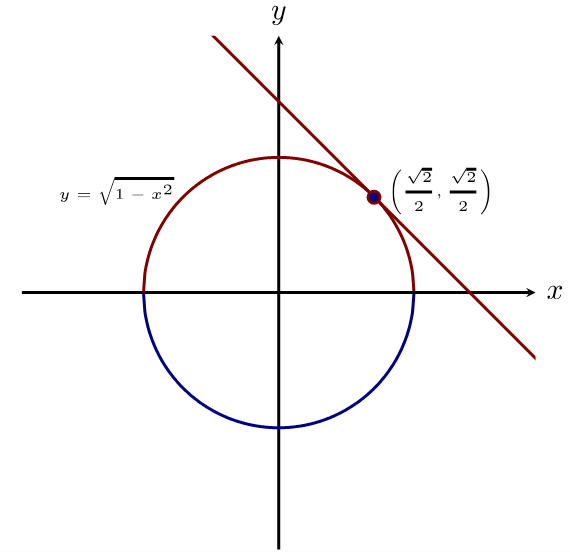
\includegraphics{0.png}
\end{image}

Once the parameter $t$ has reached $2\pi$, the circle has been traced out exactly once.



%Note that if we let $t$ continue to vary past $2\pi$ then we would start tracing out the circle again. For example, if we let $t$ run from $0$ to $6\pi$ then the circle would be traced out three complete times.
%
% Again we see the advantage of a parametric description. We could imagine a particle moving in a circular fashion in periodic motion. A Cartesian description would simply see the set of points the particle moved through. The dynamic description given by parametric equations can include information about how many times the particle has traced over that curve.

\end{example}

\begin{definition}
The direction in which the curve is traced out as the parameter increases is called the \dfn{positive orientation}.
\end{definition}



\begin{question}
In the example of the circle above, what is the positive orientation?

\begin{multipleChoice}
\choice {clockwise}
\choice[correct] {counterclockwise}
\end{multipleChoice}
\end{question}


Using parametric equations allows us to describe many curves which would be too difficult to describe otherwise.


\begin{example}
Consider the following parametric equations where $0 <t < 8\pi$.

\[
\begin{cases}
x(t)&=t\cos(t) \\
y(t)&=t\sin(t)
\end{cases}
\]

As the parameter increases, the curve rotates like it will trace out the circle. However instead of having a fixed amplitude that describes how far the circle is from the origin, the $t$ factor in front of the cosine and sine term can be thought of as a varying radius that increases as $t$ increases. Thus as the parameter increases, the curve rotates in a counterclockwise fashion like the circle but with a radius that keeps getting larger and larger. This leads to the following spiral shape.

\begin{image}
  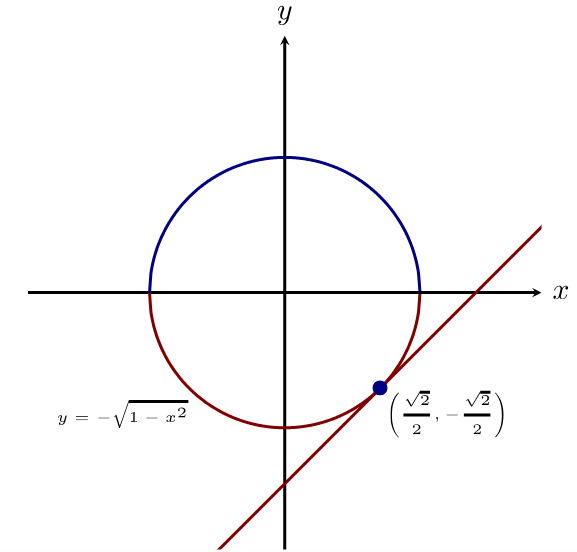
\includegraphics{1.png}
\end{image}

\end{example}

\begin{question}
  Do the parametric equations

\[
\begin{cases}
x(t)&=t\cos(t) \\
y(t)&=t\sin(t)
\end{cases}
\]
  as $t$ runs from $0$ to $2\pi$ define a function of $t$?
  \begin{multipleChoice}
    \choice{No, because the graph does not pass the vertical line
      test.}
    \choice[correct]{Yes, it is a function of $t$, because for each input
      $t$, there is exactly one output value, an ordered pair.}
  \end{multipleChoice}
  \begin{feedback}
    For the graph of a circle, $y$ is \textbf{not} a function of
    $x$. However, it can be a function of $t$ that maps
    \begin{align*}
    \R &\to \R\times \R\\
    t &\mapsto (x,y)
    \end{align*}
    where the domain is $[0,2\pi)$ and the elements of the range
      consist of ordered pairs.
  \end{feedback}
\end{question}


%
%One important class of parametric curves are \dfn{Lissajous figures}. These are curves of the form
%\begin{align*}
%  x(t) &= A \sin(at + \delta)\\
%  y(t) &= B\sin(bt)
%\end{align*}
%Here is a plot of a Lissajous curve where $A=B=1$, $\delta = \pi/2$,
%$a=5$ and $b=4$
%\begin{image}
%\begin{tikzpicture}
%	\begin{axis}[
%            %xmin=-25,xmax=25,ymin=-25,ymax=25,
%            width=3in,
%            clip=false,
%            axis lines=center,
%            %ticks=none,
%            unit vector ratio*=1 1 1,
%            xlabel=$x$, ylabel=$y$,
%            every axis y label/.style={at=(current axis.above origin),anchor=south},
%            every axis x label/.style={at=(current axis.right of origin),anchor=west},
%          ]
%          \addplot [very thick, penColor, smooth,samples=100,domain=(0:2*pi)] ({cos(deg(5*x))},{sin(deg(4*x))});
%        \end{axis}
%\end{tikzpicture}
%\end{image}
%These figures come up a lot in electrical engineering. Do yourself a
%favor and play around with Lissajous figures for differing values of
%$\delta$, $a$ and $b$.



\section{Projectile Motion}

Parametric descriptions of curves occur in many applications. For example, in physics, a common scenario is to have a object acted upon by forces. We use information about the initial state of the system as well as the laws of motion to solve for how the object will behave. This description will naturally be equations which describe how the position of the object, in a coordinate system, will change with time. Therefore, parametric descriptions of curves are very natural way to describe the motion of objects. Although we will focus on describing curves parametrically in the plane, the ideas we cover can be easily generalized to three dimensions and higher.



\begin{example}

 In differential calculus, you likely discussed projectile motion in one dimension. For example, suppose you launch a ball straight up into the air. You then want to find the position
$y(t)$ of the object with respect to time. Using integration and the fact that the ball has a constant acceleration with respect to gravity, we can find the trajectory of the ball.

\begin{explanation}
We choose the $y$-axis so that the origin is at ground level and the positive direction on the $y$-axis is upward.

Now the acceleration due to gravity is constant and we take $g=-9.8$ $m/s^2$. Call the initial velocity $v_{0y}$ (this is the intial velocity in $y$ direction). Then we can integrate and use the intial velocity to find the velocity $v(t)$
\[
v(t)=\answer[given]{-9.8}t+v_{0y}
\]

\begin{hint}
Compute $\int -9.8 \d t$ with initial condition $v(0)=v_{0y}$.
\end{hint}

Suppose it is launched from a height $y_{0}$. Integrating again and using the intial position, we obtain

\[
y(t)=\answer[given]{-4.9}t^2+v_{0y}t+ \answer[given]{y_{0}}
\]

\end{explanation}

Now suppose we want to launch the ball at an angle instead of straight up.  The ball's path will have both a vertical and horizontal component, so this is now a two dimensional problem. We launch our ball with a certain initial speed $v_{0}$. We again choose a coordinate system. Choose the origin at a fixed point on the ground level, choose the $y$-axis oriented upward, and choose our $x$-axis to be the direction in which we launch our projectile. Ignoring air resistance, the trajectory of our object will be confined to this $xy$-plane. Suppose our object is launched from an initial position $(x_{0},y_{0})$ in our coordinate system.  Can we describe the motion of the ball?

\begin{explanation}

It turns out the motion of the object can be analyzed in the $x$ and $y$ directions separately.  We can describe the position of the ball as

\[
\begin{cases}
x&=x(t) \\
y&=y(t)
\end{cases}
\]

The angle that we launch our ball determines an the initial velocity $v_{0}$ in each components. Take $v_{0y}$ to be the initial velocity  along the $y$ direction and $v_{0x}$ to be the initial velocity along the $x$ direction. In the $y$ direction, our ball will behave just like a ball thrown straight upwards. Using our previous work on one dimensional projectile motion, we obtain

\[
y(t)=-4.9t^2+v_{0y}t+y_{0}
\]

Now we want to understand the behavior in the $x$ direction. There are no forces in the $x$ direction so the acceleration is $0$.   Using the initial velocity  $v_{0x}$ in the $x$ direction and integrating the acceleration $a_{0x}=0$, we find $v(t)=v_{0x}$.  Integrating again and using the initial $x$ position $x_{0}$, we obtain
$x(t)$:

\[
x(t)=v_{0x}t+x_{0}
\]

This gives us the parametric description of the trajectory of the ball in the $xy$ plane with respect to time.

\[
\begin{cases}
x(t)&=v_{0x}+x_{0}\\
y(t)&=-4.9t^2+v_{0y}t+y_{0}
\end{cases}
\]

The curve that the projectile follows is parabolic. However the parametric description gives us more information. It gives us a dynamic description that tells us the position of the particle at each moment of time.

\end{explanation}

\end{example}



\begin{onlineOnly}
\desmos{i8vl8gblrg}{1024}{500}



Explore changing the initial velocities $v_{0x}$ and $v_{0y}$  in the $x$ and $y$ directions and see how that changes the trajectory of the ball by use the slider $a$ to trace the curve.
\end{onlineOnly}










\section{Multiple parametrizations of a given curve}

Given a curve $C$, there are many different sets of parametric equations that trace out $C$.


Previously we saw that we can parametrize the circle as

\[
\begin{cases}
x(t)&=\cos(t) \\
y(t)&=\sin(t)
\end{cases}
\]
as $t$ varies over the interval $[0, 2\pi)$, traces out the circle in a counterclockwise fashion.

Suppose we replace $t$ by $-t$ in these equations.

\[
\begin{cases}
x(t)&=\cos(-t) \\
y(t)&=\sin(-t)
\end{cases}
\]

where $t$ runs over the interval $[0, 2\pi)$. Let's make a table.

\[
\begin{array}{c|c|c}
  t  & x =\cos(-t) & y = \sin(-t)\\\hline
  0  & 1  & 0 \\
  \pi/6  & \sqrt{3}/2 & -1/2 \\
  \pi/4  & -4 & 7 \\
  \pi/3  & -7 & 11\\
  \pi/2  & -10& 15
\end{array}
\]
%Finish this table!

Now the positive orientation of the curve is clockwise.  Notice that if we replace $t$ by any expression in $t$, we will trace out (a portion of) the same curve, but possibly at a different speed and/or in a different direction.

\begin{question}
  Which of the following parametric equations draw the line $y=x$?
  \begin{selectAll}
    \choice[correct]{$x(t) = t$ and $y(t) = t$ for $-\infty < t < \infty$}
    \choice[correct]{$x(t) = t-5$ and $y(t) = t-5$ for $-\infty < t < \infty$}
    \choice{$x(t) = \sin(t)$ and $y(t) = \sin(t)$ for $-\infty < t < \infty$}
    \choice[correct]{$x(t) = \tan(t)$ and $y(t) = \tan(t)$ for $-\pi/2 < t < \pi/2$}
    \choice{$x(t) = t^2$ and $y(t) = t^2$ for $-\infty < t < \infty$}
    \choice[correct]{$x(t) = t^3$ and $y(t) = t^3$ for $-\infty < t < \infty$}
  \end{selectAll}
\end{question}


\begin{question}
  Which of the following parametric equations draw the circle $(x-1)^2
  + (y-2)^2 = 3^2$?
  \begin{selectAll}
    \choice[correct]{$x(t) = 1 + 3\cos(t)$ and $y(t) = 2 + 3\sin(t)$ for $0 \le t \le 2\pi$}
    \choice[correct]{$x(t) = 1 + 3\cos(t)$ and $y(t) = 2 + 3\sin(t)$ for $2\pi \le t \le 4\pi$}
    \choice[correct]{$x(t) = 1 + 3\sin(t)$ and $y(t) = 2 + 3\cos(t)$ for $0 \le t \le 2\pi$}
    \choice{$x(t) = 2 + 3\sin(t)$ and $y(t) = 1 + 3\cos(t)$ for $0 \le t \le 2\pi$}
    \choice{$x(t) = 1 + 3\cos(e^t)$ and $y(t) = 2 + 3\sin(e^t)$ for $0 \le t \le \ln(2\pi)$}
    \choice[correct]{$x(t) = 1 + 3\cos(e^t)$ and $y(t) = 2 + 3\sin(e^t)$ for $\ln(2\pi) \le t \le \ln(4\pi)$}
  \end{selectAll}
\end{question}











\section{When is it easy to find a parametrization of a curve?}

Suppose you are given a curve $C$ and you want to find a parametrization for $C$. There are certain nice curves where we can easily come up with an explicit parametrization.

\subsection{Graphs of functions}

If you are given the graph of a function $y=f(x)$ then it is easy to find a parametric description of the curve. The key idea is that the independent variable is already acting like a parameter so we can use


\[
\begin{cases}
x(t)&=t \\
y(t)&=f(t)
\end{cases}
\]

In this way, we can easily parametrize any curve given as the graph of a function.

\begin{question}
  Can you use the technique described immediately above to express $y
  = e^x$ as a parametric function?
  \begin{prompt}
    \begin{align*}
      x(t) &= \answer{t}\\
      y(t) &= \answer{e^t}
    \end{align*}
  \end{prompt}
\end{question}


\subsection{Lines}

Suppose we are given two points $p_{1}=(a,b)$ and $p_{2}=(c, d)$. Suppose we are interested in parametrizing the line segment from $p_{1}$ to $p_{2}$. There is a canonical way to parameterize the line segment so that the parameter is $0$ at $p_{1}$ and is equal to $1$ at $p_{2}$. In a previous example, we have seen that if both $x(t)$ and $y(t)$ are lines then the curve traced out is a line. Thus it suffices to construct a line $x(t)$ so that $x(0)=a$ and $x(1)=c$. Similarly we construct a line $y(t)$ so that $y(0)=b$ and $y(1)=d$. This
 leads to the equations


\[
\begin{cases}
x(t)&=a+t(c-a) \\
y(t)&=b+t(d-b)
\end{cases}
\]
where we let $t$ vary over the interval $[0,1]$.

If we let $t$ vary over the entire real line in this example, then we get the unique line that passes through the points $p_{1}$ and $p_{2}$.

\begin{question}
Use this method to find a parametric equation for a line segment that starts at the point $(2,1)$ and ends at the point $(8, 5)$.

Let
\[
\begin{cases}
x(t)&=\answer{2+6t}\\
y(t)&=\answer{1+4t}
\end{cases}
\]
for $t$ in the interval $[0, 1]$.


\end{question}




\subsection{Circles}

The \dfn{standard form for a circle} centered at a point $(a,b)$ with
radius $r$ is given by
\[
(x-a)^2 + (y-b)^2 = r^2.
\]
One problem with the standard form for a circle is that it is somewhat
difficult to find points on the circle. A parametric equation
representing a circle solves this problem.

\begin{example}
  Give a parametric equation representing the circle
  \[
  (x-1)^2 + (y-2)^2 = 3^2
  \]
  and explain why your answer is correct.
  \begin{explanation}
    This is the circle of radius $3$ centered at the point
    $(1,2)$. Here we set
    \begin{align*}
      x(t) &= \answer[given]{1} + \answer[given]{3}\cos(t)\\
      y(t) &= \answer[given]{2} + \answer[given]{3}\sin(t)
    \end{align*}
    as $t$ runs from $0$ to $2\pi$.  To see that our answer is
    correct, we can ``plug'' it back into the implicit equation
    for the circle. Write with me:
    \begin{align*}
      (x-1)^2 + (y-2)^2 &= (x(t)-1)^2 + (y(t)-2)^2\\
      &= (1 + 3\cos(t)-1)^2 + (2 + 3\sin(t)-2)^2\\
      &= (3\cos(t))^2 + (3\sin(t))^2\\
      &= 3^2\cos^2(t) + 3^2\sin^2(t)\\
      &= 3^2(\cos^2(t) + \sin^2(t))\\
      &= 3^2
    \end{align*}
    by the Pythagorean identity.\index{Pythagorean identity} Since our
    functions $(x(t),y(t))$ satisfy the form of the circle, our
    solution is correct.
  \end{explanation}
\end{example}





    \begin{question}
      One day while trying to graph a unit circle, you accidentally
      write down
      \begin{align*}
        x(t) &= \sin(t)\\
        y(t) &= \cos(t)
      \end{align*}
      What happens now? Do you still get a circle? How is this different
      from what we did in the previous question?
      \begin{prompt}
        \begin{multipleChoice}
        \choice{you still plot a unit circle in a counterclockwise fashion, with the same starting and ending points}
        \choice{you plot a unit circle but in a clockwise fashion, with the same starting and ending points}
        \choice{you still plot a unit circle in a counterclockwise fashion, but the starting and ending points are different}
        \choice[correct]{you plot a unit circle but in a clockwise fashion, but the starting and ending points are different}
        \choice{this no longer plots a circle}

        \end{multipleChoice}
      \end{prompt}
  \end{question}


In mathematics, when parameterizing closed curves (like circles), the
convention is to draw them in a ``counterclockwise'' direction. This
is called the \dfn{positive orientation}.

\begin{warning}
  If you parameterize your closed curves in a clockwise direction, you
  may find your ``answers'' are off by a factor of $-1$.
\end{warning}

\begin{question}
What should $x(t)$ and $y(t)$ be to parameterize the circle
\[
(x-a)^2 + (y-b)^2 = r^2.
\]
in a counterclockwise fashion, with $t=0$ corresponding to $(1,0)$?
\begin{prompt}
  \begin{align*}
    x(t) &= \answer{a} + \answer{r}\cdot \cos(t)\\
    y(t) &= \answer{b} + \answer{r}\cdot \sin(t)
  \end{align*}
\end{prompt}
\end{question}




\section{Converting from parametric to cartesian }

We mentioned earlier that graphing a curve from a  given set of parametric equations directly from can be quite difficult. Usually computational software is needed. However there are some occasions where we can eliminate the parameter and obtain an equation involving only $x$ and $y$.

Here are some basic strategies to try:
\begin{itemize}
\item Solve for $t$.
\item Solve for a function of $t$.
\item Use a trigonometric identity.
\end{itemize}
In each case the process that we are using is called
\dfn{elimination of a parameter}.

We'll give several examples of how one actually \textit{eliminates a
  parameter}.

\subsection{Solving for the variable}

In the first example, we'll solve for $t$.
\begin{example}
  Let
  \begin{align*}
    x(t) &= -4 t^2\\
    y(t) &= 3t-1.
  \end{align*}
    Eliminate a parameter to express this curve purely in terms of $x$ and $y$.
  \begin{explanation}
    Here we will solve for $t$. Since it is easier, we will solve for
    $t$ in this equation:
    \begin{align*}
      y &= 3t-1\\
      y+1 &= \answer[given]{3t}\\
      \frac{y+1}{3} & = \answer[given]{t}.
    \end{align*}
    Now plug this into $x(t) = -4 t^2$, and write
    \[
    x = \answer[given]{-4 \left(\frac{y+1}{3}\right)^2}.
    \]
  \end{explanation}
\end{example}

We see in this situation that the set of points traced out the curve (as we vary over all possible values of $t$) is a parabola.

\subsection{Solving for a common function}

Sometimes instead of solving for the parameter directly, it is easier to solve for a function of the parameter that is common to both $x(t)$ and $y(t)$.

\begin{example}
  Let
  \begin{align*}
    x(t) &= -5e^t\\
    y(t) &= e^{3t}.
  \end{align*}
    Eliminate a parameter to express this curve purely in terms of $x$
    and $y$.
    \begin{explanation}
      Here we will solve for a function of $t$. Write
      \begin{align*}
        x &= -5e^t\\
        \frac{x}{-5} &= e^t
      \end{align*}
      Now we can rewrite $y(t)$ as
      \begin{align*}
        y(t) &= e^{3t}\\
        y(t) &= \left(e^{t}\right)^{\answer[given]{3}}.
      \end{align*}
      Now we see that
      \[
      y = \answer[given]{\left(\frac{x}{-5}\right)^3}.
      \]
  \end{explanation}
\end{example}


\subsection{Solving for related functions}



\begin{example}
  Let
  \begin{align*}
    x(t) &= 3\cos(t)\\
    y(t) &= 1+4\sin(t).
  \end{align*}
  Eliminate a parameter to express this curve purely in terms of $x$ and $y$.
  \begin{explanation}
    There is no common function of $t$ in the two equations. Furthermore solving for $t$ directly is possible but there is a easier path forward. Notice that if we rearrange the equations slightly, then we can make use of a trig identity to eliminate the expressions involving $t$.  We use the Pythagorean identity:
    \[
    \cos^2(t) + \sin^2(t) = 1
    \]
    So first isolate cosine and sine, and square the equations. With $x(t)$ we have
    \begin{align*}
      x &= 3 \cos(t) \\
      \answer[given]{\frac{x}{3}} &= \cos(t)\\
      \answer[given]{\left(\frac{x}{3}\right)^2} &= \cos^2(t)
    \end{align*}
    and with $y(t)$ we have
    \begin{align*}
      y &= 1 + 4\sin(t)\\
      y-1 &= 4\sin(t)\\
      \frac{y-1}{4} &= \sin(t)\\
      \left(\frac{y-1}{4}\right)^2 &= \sin^2(t).
    \end{align*}
    Plugging this back into the Pythagorean identity, we see:
    \begin{align*}
      \cos^2(t) + \sin^2(t) &= 1\\
      \left(\frac{x}{3}\right)^2 + \left(\frac{y-1}{4}\right)^2 &= 1.
    \end{align*}
  \end{explanation}
\end{example}

These techniques are useful to know since they can help you more easily visualize certain simple parametric curves. However, when you eliminate the parameter it is important to realize that you are losing information about how the curve is traced out.
\end{document}
